\documentclass[twoside,english]{uiofysmaster}

\usepackage[utf8]{inputenc} % Riktig tegnsett
\usepackage{babel} 
\usepackage{url}
\usepackage{units}
\usepackage{lipsum}
\usepackage{graphicx}  
\usepackage{subcaption} 
\usepackage{color}
\usepackage{amsmath}  
\usepackage{hyperref}
\usepackage{braket} 
\usepackage{multicol}
\usepackage{listings}  
\usepackage{amsfonts}
\usepackage{siunitx}
\usepackage{float}
\usepackage{minted}
% Custom commands
\newcommand\lr[1]{\left(#1\right)} 

\definecolor{LightBlue}{rgb}{0.8, 0.8, 0.95}

\definecolor{editColor}{rgb}{0.5, 0.0, 0.0}


\author{Filip Henrik Larsen}
\title{Title of the master thesis}
\date{May 2017}

\begin{document}

\maketitle

\begin{abstract}
This is an abstract text.
\end{abstract}

\begin{dedication}
  To someone
  \\\vspace{12pt}
  This is a dedication to my cat.
\end{dedication}

\begin{acknowledgements}
  Flora Joelle Larsen\\*
  Anders Hafreager
\end{acknowledgements}

\tableofcontents

\chapter{Introduction}

Why is the subject of this thesis of any interest?\\
What is our take on the problem?\\
What do we hope to accomplish?\\
How will this be of any contribution to anything?\\
How is the thesis laid out?

\chapter{Setting up the system}

We wish to construct a system consisting of {\color{red} two} elements made out of silica: a slab and a sphere cap. In order to do this we need to generate the spacial position coordinates (x,y,z) of every single atom. Considering that we are making a system consisting of about $10^5$ atoms, this is obviously not done manually. We have chosen to use a tool named \textit{Moltemplate}\footnote{\href{http://www.moltemplate.org/index.html}{http://www.moltemplate.org/index.html}}, which is included in the LAMMPS distribution.

The main idea is to manually enter the coordinates of only the atoms in a unit cell of the material one wish to generate, and then simply copy this unit cell wherever desired. The software will shift the coordinates of the copied unit cell by the displacement from the original image. In addition it will generate files containing data such as which atoms they share bonds with, if any, and angles between such bonds. 


\section{Silica}
Silica is a chemical compound also known as Silicon dioxide, having the chemical formula SiO$_2$. It has several polymorph structures, the most common being quartz, which is one of the most abundant minerals in the Earth's crust. Other polymorphs include cristobalite, tridymite, coesite and more.    

For our purpose it is insignificant which one we choose. Once the material is melted, it is indifferent which configuration we started from, as long as the density is correct.
In this project we will build the constituents of the system from a type of cristobalite named $\beta$-cristobalite. This is mainly because it has a simple structure and a cubical unit cell.


\subsection{Unit cell of $\beta$-cristobalite}
In order to construct the unit cell of a material, one should look up the coordinates of the atoms in a crystallography database. We have used the unit cell of $\beta$-cristobalite found at \textit{Crystallography Open Database}\footnote{\href{http://www.crystallography.net/cod/1010944.html}{http://www.crystallography.net/cod/1010944.html}}. At this site one can download a \texttt{.cif}-file consisting of the spatial positions of each atom, the length of the unit cell edges and angles between faces of the cell. In the case of $\beta$-cristobalite the unit cell is cubical with edges of length 7.12Å. It contain 8 silicon atoms and 16 oxygen atoms. The density of the unit cell can easily be computed and is 2.2114 g/cm$^3$.

\begin{figure}
	\centering
	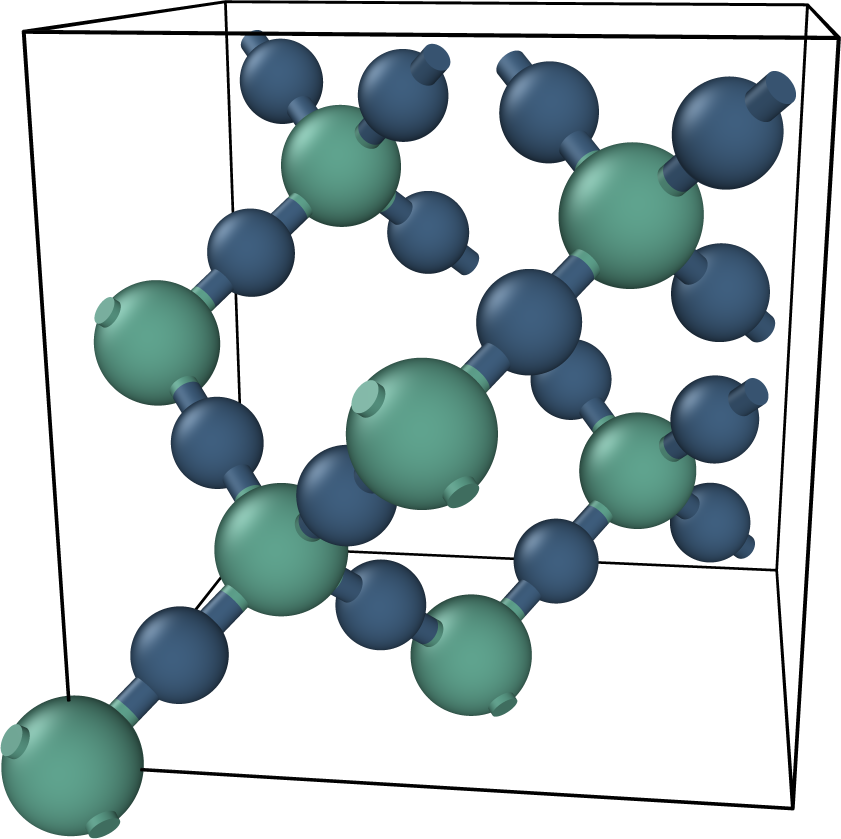
\includegraphics[width=0.7\linewidth]{figures/unitcell/unitcell.png}
	\caption{Unit cell of b-cristobalite. Tan and blue spheres represent silicon and oxygen atoms respectively.}
	\label{fig:unitcellbcristobalite}
\end{figure}



\section{Building a crystal}
The coordinates gotten from the \texttt{.cif}-file can now be implemented into \textit{moltemplate} together with whatever bond and angle data required by the potential. In our simulations we will use the Vashishta potential, which does not require these. 

Moltemplate has its own structure and syntax. The first step to build up a larger material is, as mentioned, to create the unit cell. Data concerning the unit cell are placed in a \texttt{.lt}-file, which is readable by Moltemplate. Such a file is shown in Listing \ref{lst:beta-cristobalite.lt}. 

For a more profound understanding of the structure and syntax of these files, the reader is advised to read the moltemplate manual  



\lstinputlisting[language=LammpsData]{../SiO2/beta-cristobalite.lt}

We use the unit cell as building blocks, placing them concurrently until we have a crystal of the desired size. For our purpose, we generate a large cube of $15\times15\times15$ unit cells. This is done as follows.

\begin{listing}[H]
	\inputminted[linenos, xleftmargin=6mm, bgcolor=LightBlue, fontsize=\footnotesize]{text}{../SiO2/setup.lt}
	\caption{Typical moltemplate file containing unit cell data. The columns of the "Data Atoms" section hold, from left to right, information of atom ID, atom type, x-, y- and z-position. The "Data Masses" section stores the weight of silicon and oxygen atoms in atomic mass units. }
	\label{lst:beta-cristobalite.lt}
\end{listing}


\begin{figure}
	\centering
	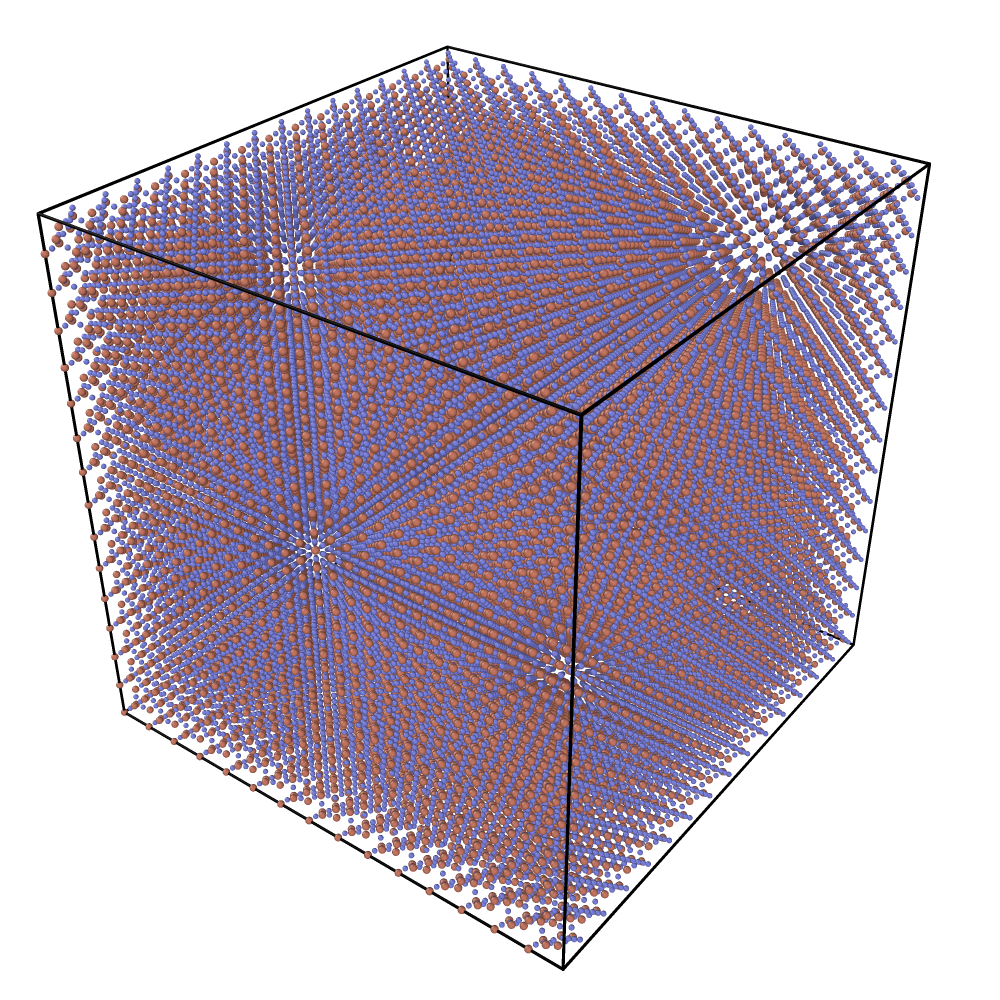
\includegraphics[width=0.7\linewidth]{figures/CreatingSystem/hugeCube}
	\caption{System built from $15\times15\times15$ unit cells of b-cristobalite.}
	\label{fig:hugeCube}
\end{figure}

\section{Shaping the silica}

\begin{figure}
	\centering
	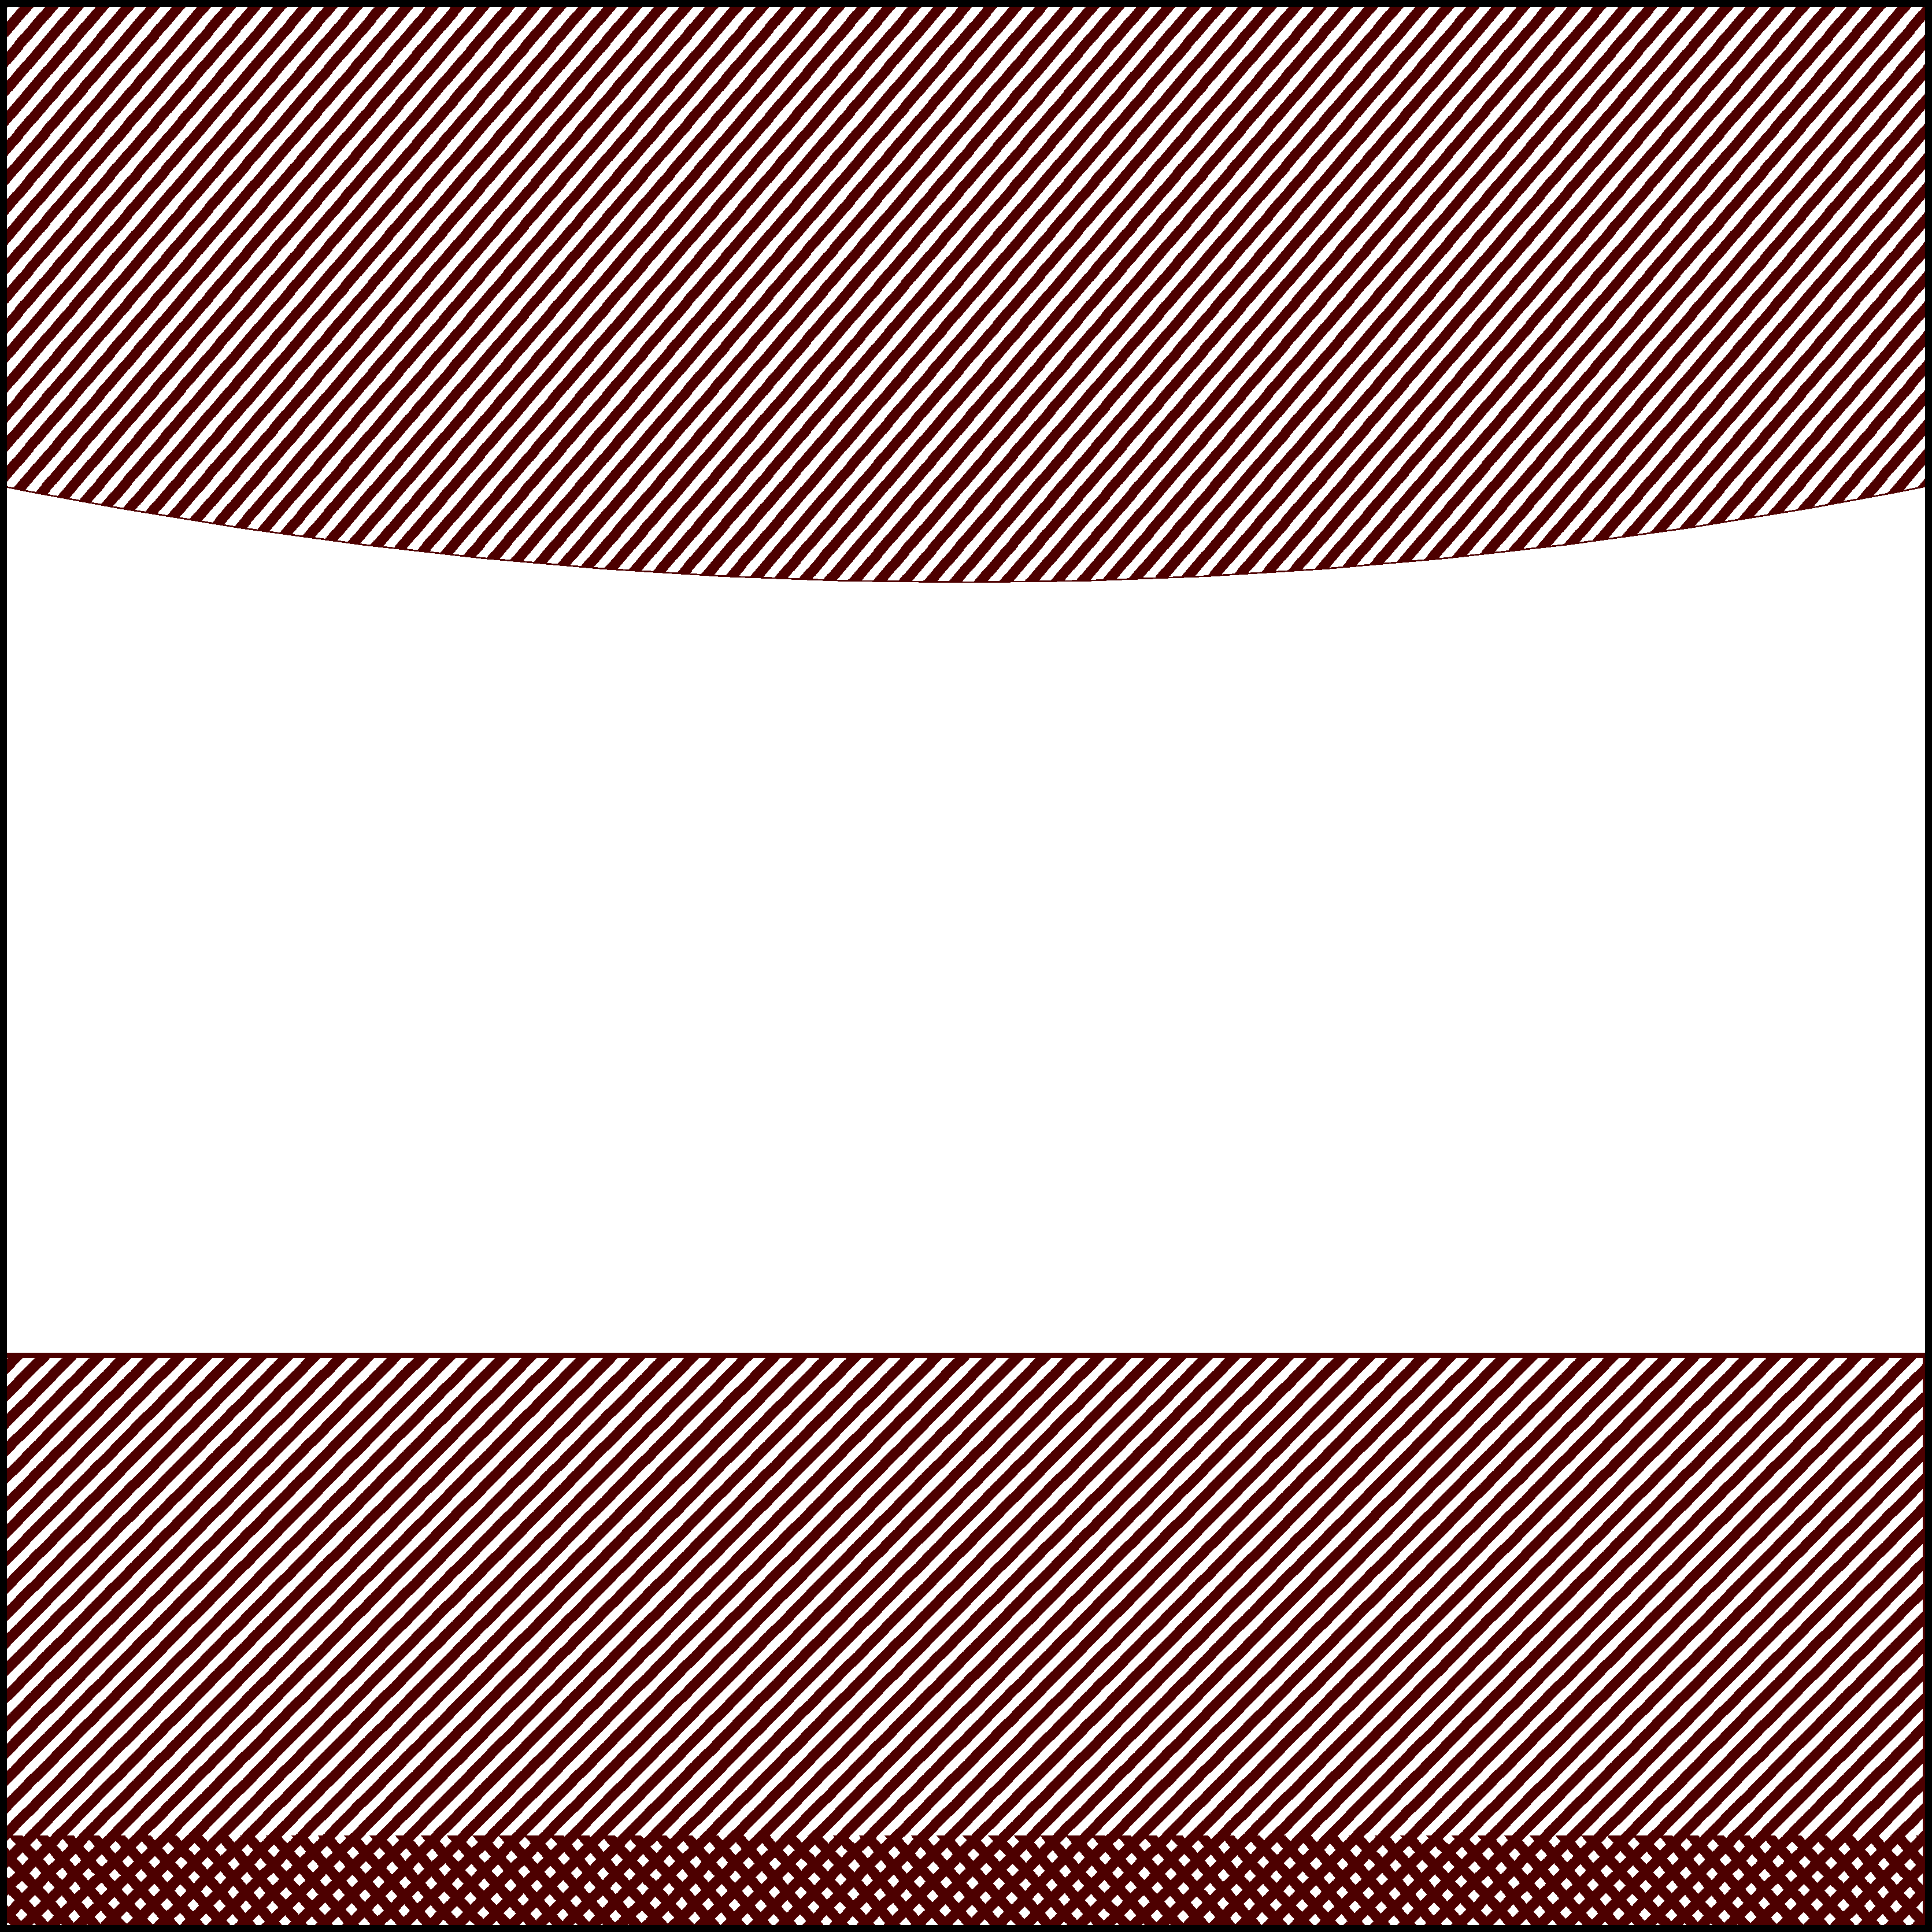
\includegraphics[width=0.7\linewidth]{figures/CreatingSystem/drawing.pdf}
	\caption{Illustrative drawing of what how the system should look. Red parallel stripes symbolize areas of silica. Red crossing stripes indicate areas of frozen silica. The boundaries are periodic in all dimensions, causing both the slab and the sphere to be connected to the frozen silica through the z-boundaries.}
	\label{fig:drawing}
\end{figure}

The huge cube of silica can be carved however we like by defining regions from which we delete the containing atoms. In LAMMPS this is done by using the \texttt{region}, \texttt{union}, \texttt{intersect} and \texttt{delete atoms} commands. Our implementation is stated in Listing \ref{lst:sculpting}, which is very simple due to the way we are going to treat the boundary conditions. 
\begin{listing}
	\inputminted[linenos, xleftmargin=6mm, bgcolor=LightBlue, fontsize=\footnotesize]{bash}{../SiO2/system.prepare.latex}
	\caption{Defining regions to keep or delete from a system of dimensions $106.8\times106.8\times106.8$ Å.}
	\label{lst:sculpting}
\end{listing}








\bibliography{resources/Library.bib}


%Referances






\end{document}
```

Centering the front page
------------------------
By default, the maketitle command will generate the front page, but it will not be properly centered, but offset like any other page. To get around this, the best solution is to create a separate document, name it front-page.tex and add the following to it:

front-page.tex:
```latex
\documentclass[twoside,english]{uiofysmaster}
\geometry{a4paper,includeall,bindingoffset=0cm,margin=3cm,
            marginparsep=0cm,marginparwidth=0cm,top=2cm}

\author{Filip Henrik Larsen}
\title{\uppercase{The history of master thesises and other random gibberish}}
\date{June 2012}

\begin{document}

\begin{titlepage}
\maketitle
\end{titlepage}

\end{document}
